\chapter{\IfLanguageName{dutch}{Stand van zaken}{State of the art}}
\label{ch:stand-van-zaken}

\section{Inleiding}
In dit hoofdstuk wordt een overzicht gegeven van de huidige stand van zaken rondom mobiele applicatieontwikkeling. De focus ligt daarbij op beveiliging, de keuze van platformen en cross-platform technologieën. Het doel is om de technologische context van dit project helder in kaart te brengen, zodat er een weloverwogen keuze kan worden gemaakt voor het meest geschikte ontwikkelplatform. Door recente ontwikkelingen en relevante literatuur te bespreken, leggen we een stevige basis voor de onderzoeksvragen en ontwerpbeslissingen die hierop volgen.

\section{Vergelijking van mobiele ontwikkelstrategieën}
Mobiele applicaties kunnen op verschillende manieren ontwikkeld worden, elk met hun eigen voor- en nadelen. De drie meest gebruikte strategieën zijn native apps, Progressive Web Apps (PWA’s) en cross-platform frameworks. In deze sectie worden deze benaderingen apart besproken, waarna ze vergeleken worden op punten als prestaties, gebruikservaring en ontwikkeltijd.

\subsection{Native apps}
Native apps worden specifiek ontwikkeld voor één platform, zoals Android of iOS. Dit gebeurt met platformgebonden programmeertalen en tools, bijvoorbeeld Kotlin of Java voor Android, en Swift of Objective-C voor iOS. Volgens \textcite{Gillis} levert deze aanpak de beste prestaties en de diepste integratie met het besturingssysteem, inclusief directe toegang tot hardware en native UI-elementen.

Een belangrijk voordeel is dat native apps een optimale gebruikerservaring bieden: ze voelen als een natuurlijk onderdeel van het platform, laden snel, tonen vloeiende animaties en volgen consistente interactiepatronen \textcite{Gillis}. Daartegenover staat dat deze aanpak vaak aparte ontwikkelteams per platform vereist, wat kan leiden tot hogere kosten en een langere time-to-market.

\subsection{Progressive Web Apps (PWA)}
Progressive Web Apps zijn webapplicaties die zich gedragen als native apps. Ze maken gebruik van moderne webtechnologieën zoals HTML5, CSS3 en JavaScript, in combinatie met service workers en manifest-bestanden. PWA’s draaien in een browseromgeving, maar kunnen ook offline functioneren, pushnotificaties versturen en op het startscherm van een toestel worden geplaatst.

De belangrijkste voordelen van PWA’s zijn hun platformonafhankelijkheid en relatief lage ontwikkelkosten: één codebase is voldoende voor alle apparaten met een moderne browser. De functionaliteit is echter beperkter dan bij native apps, vooral wat betreft toegang tot hardware en beveiligde API’s. Zo is de ondersteuning voor pushnotificaties en offline opslag op iOS nog steeds minder uitgebreid dan op Android.

De markt voor PWA’s groeit snel. In 2023 werd de wereldwijde marktwaarde geschat op 1,46 miljard USD, met een verwachte jaarlijkse groei van 31,1 procent tussen 2024 en 2030 \autocite{Research2024}. Deze groei wordt gedreven door factoren zoals de toenemende internetpenetratie en de vraag naar snelle, toegankelijke mobiele ervaringen. Grote bedrijven zoals Tinder, X (voorheen Twitter) en Forbes maken al gebruik van PWA-technologie. Figuur~\ref{fig:pwa_market} toont de verwachte marktgroei tot 2030.

\begin{figure}[h]
    \centering
    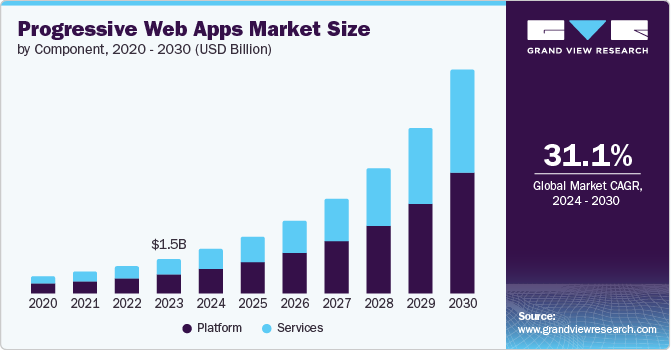
\includegraphics[width=0.75\textwidth]{pwa-market.png}
    \caption{Wereldwijde marktgroei van Progressive Web Apps (USD miljard), 2020–2030. Bron: Grand View Research, 2025. \autocite{Research2024}}
    \label{fig:pwa_market}
\end{figure}

\subsection{Cross-platform frameworks}
Cross-platform frameworks zoals Flutter, React Native en .NET MAUI vormen een middenweg tussen de prestaties van native apps en de snelle ontwikkeltijd van PWA’s. Ze maken het mogelijk om met één gedeelde codebase applicaties te ontwikkelen voor meerdere platformen, wat de ontwikkeltijd verkort en onderhoudskosten verlaagt \autocite{Kuppan2024}.\\

Flutter en React Native gebruiken eigen rendering-engines of native componenten voor de gebruikersinterface, terwijl .NET MAUI direct platform-native UI-elementen aanspreekt via .NET-technologie. Uit onderzoek blijkt dat Flutter uitblinkt in vloeiende animaties en UI-prestaties, terwijl .NET MAUI sterk is in integratie met Microsoft-omgevingen \autocite{Gajjam2025}. Toch blijven cross-platform apps soms iets achter bij native apps, vooral bij grafisch intensieve of rekenintensieve toepassingen.

\begin{table}[h]
    \centering
    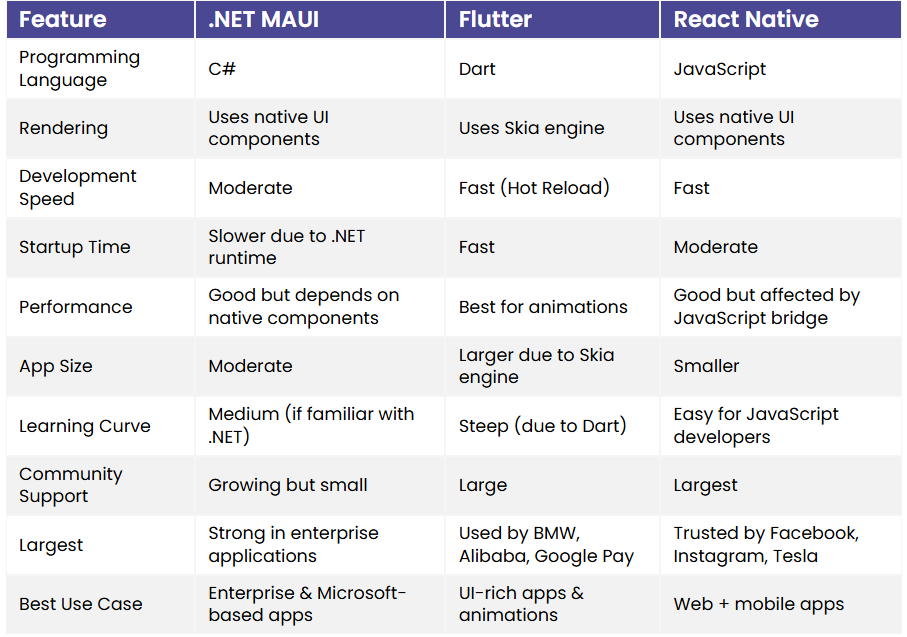
\includegraphics[width=0.8\textwidth]{comparison1.png}
    \caption[Integratie]{Vergelijking van .NET MAUI, Flutter en React Native op basis van geschiktheid voor enterprise-omgevingen \autocite{Gajjam2025}}
    \label{fig:vergelijking}
\end{table}

\begin{table}[h]
    \centering
    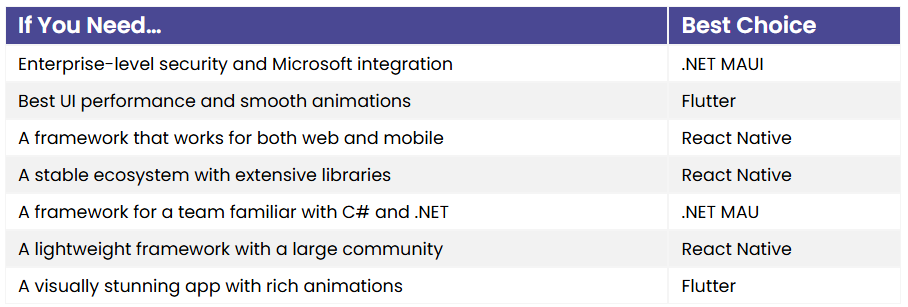
\includegraphics[width=0.8\textwidth]{comparison2.png}
    \caption[Frameworkkeuze]{Overzicht van aanbevolen cross-platform frameworks (Flutter, React Native en .NET MAUI) op basis van specifieke projectvereisten \autocite{Gajjam2025}}
    \label{tab:frameworkkeuze}
\end{table}

\subsection{Samenvatting en aanbevelingen}
Welke mobiele ontwikkelstrategie het beste past, hangt af van de context, de doelstellingen en de technische randvoorwaarden van het project. Native apps zijn ideaal voor toepassingen waarbij maximale prestaties en een hoogwaardige gebruikerservaring cruciaal zijn, bijvoorbeeld bij games of apps met intensieve interactie. Deze aanpak zorgt voor optimale integratie met het besturingssysteem en directe hardwaretoegang, maar vergt vaak aparte teams per platform, wat hogere kosten en een langere ontwikkeltijd tot gevolg heeft.\\

Progressive Web Apps bieden een kosteneffectieve, platformonafhankelijke oplossing, met één codebase voor alle moderne browsers. Ze zijn geschikt voor eenvoudige of informatieve apps zonder complexe functies. De functionaliteit is echter beperkter, vooral wat betreft hardwaretoegang en beveiligde API’s. Ook is de ondersteuning voor bepaalde functies, zoals pushnotificaties op iOS, nog beperkt.\\

Cross-platform frameworks als Flutter, React Native en .NET MAUI vormen een aantrekkelijk compromis: met één gedeelde codebase kunnen apps voor meerdere platformen worden ontwikkeld, wat de ontwikkeltijd verkort en het onderhoud vereenvoudigt. Flutter onderscheidt zich door uitstekende UI-prestaties en animaties, terwijl .NET MAUI een goede keuze is voor organisaties die diep in het Microsoft-ecosysteem zitten, mede dankzij de integratie met Visual Studio en Azure.\\

Figuur~\ref{fig:vergelijking} toont een overzicht van de voor- en nadelen van deze strategieën. De beste keuze hangt af van het doel van de app, de gewenste gebruikerservaring en de beschikbare middelen. Zo is .NET MAUI vaak de beste optie in enterprise-omgevingen waar stabiliteit, veiligheid en integratie centraal staan, terwijl native ontwikkeling of PWA’s beter kunnen passen bij specifieke projectdoelen en budgetten.\\

Kortom, door zorgvuldig te wegen tussen prestaties, ontwikkeltijd, functionaliteit en organisatorische context, kan een projectteam een mobiele ontwikkelstrategie kiezen die zowel technische als zakelijke eisen optimaal bedient.

\section{Vergelijking van Cross-Platform Frameworks}

\subsection{Flutter}
Flutter is een open-source UI-framework van Google, gebaseerd op de programmeertaal Dart. Het staat bekend om hoge prestaties, vloeiende animaties en een uitgebreide set widgets voor native-achtige gebruikersinterfaces. Flutter ondersteunt iOS, Android, web en desktop en profiteert van een groeiende community met veel beschikbare plug-ins \autocite{Gajjam2025}.\\

Een onderscheidend kenmerk is \emph{hot reload}, waarmee ontwikkelaars realtime wijzigingen kunnen doorvoeren, wat de ontwikkelsnelheid sterk verhoogt. Flutter ondersteunt zowel Material Design als Cupertino-stijl en maakt gebruik van de Skia-renderengine voor consistente prestaties \autocite{Rodriguez2025}.\\

In 2023 gebruikte 46\% van ontwikkelaars wereldwijd Flutter, waarmee het het populairste cross-platform framework is. Grote merken zoals Google Ads, BMW en Alibaba vertrouwen op Flutter, wat de kracht van één codebase en besparingen in tijd en kosten benadrukt. Figuur~\ref{fig:flutter} toont een overzicht van het gebruik van verschillende frameworks.\\

\begin{figure}[h]
    \centering
    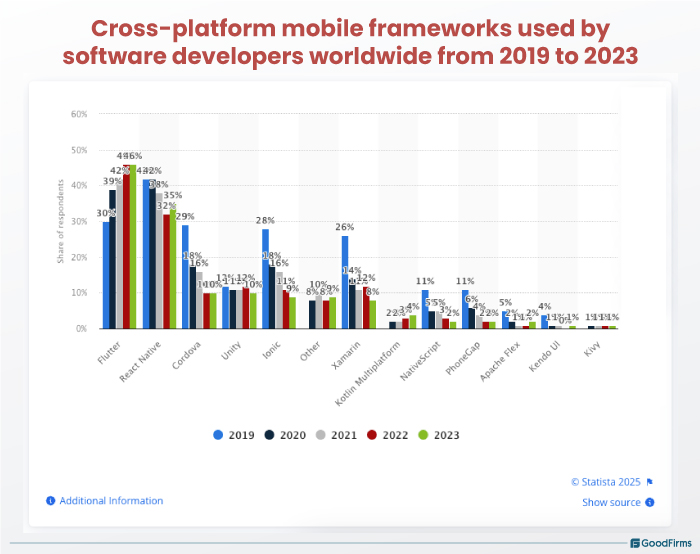
\includegraphics[width=0.75\textwidth]{flutter.jpg}
    \caption{Gebruik van cross-platform frameworks onder ontwikkelaars in 2023. Bron: Statista \autocite{Rodriguez2025}}
    \label{fig:flutter}
\end{figure}

Een beperking is de matige integratie met enterprise-systemen en Microsoft-technologieën, wat voor organisaties die sterk op het Microsoft-ecosysteem steunen een nadeel kan zijn.

\subsection{React Native}
React Native, ontwikkeld door Meta, maakt het mogelijk mobiele apps te bouwen met JavaScript en React. Het biedt een goede balans tussen snelheid, performance en schaalbaarheid, zeker in combinatie met het Expo-platform dat native build-omgevingen vereenvoudigt \autocite{Ivanov2025}.\\

Met één codebase voor iOS en Android worden ontwikkeltijden verkort en kosten gedrukt, wat vooral aantrekkelijk is voor kleine teams. Expo voegt hier hot reloading en een managed workflow aan toe, plus de Expo Go-app voor directe testing op fysieke apparaten \autocite{Ivanov2025}.\\

React Native levert native-achtige prestaties via een brug naar native API's, en animaties verlopen soepel dankzij bibliotheken als react-native-reanimated \autocite{Ivanov2025}. Over-the-Air updates maken snelle uitrol van fixes mogelijk zonder app store tussenkomst.\\

Echter, voor complexe platform-specifieke functies is vaak native code nodig, wat extra onderhoud vergt. De integratie met Microsoft-technologieën is beperkt, waardoor .NET MAUI vaak de voorkeur heeft in enterprise-omgevingen met Azure en .NET-backends \autocite{Longe2025}.

\subsection{.NET MAUI}
.NET MAUI, de opvolger van Xamarin, is Microsofts nieuwste cross-platform framework. Het stelt ontwikkelaars in staat met één codebase apps te bouwen voor iOS, Android, Windows en macOS, wat kosten en onderhoud reduceert \autocite{Sheth2024}.\\

De diepe integratie met het Microsoft-ecosysteem (Visual Studio, Azure, .NET Core) zorgt voor uniforme tooling, samenwerking en toegang tot uitgebreide documentatie \autocite{Sheth2024}. Visual Studio ondersteunt functies als Hot Reload en Live Preview voor een snelle ontwikkelcyclus.\\

Dankzij een single-projectstructuur vereenvoudigt .NET MAUI platformoverschrijdend ontwikkelen, terwijl native UI-componenten automatisch aangepast worden aan het besturingssysteem \autocite{Sheth2024}. Dit zorgt voor consistente gebruikerservaring zonder in te boeten aan merkidentiteit.\\

Performance is sterk dankzij efficiënt geheugenbeheer, snelle opstarttijden en directe toegang tot native API’s. Platform-specifieke extensies zijn mogelijk via custom handlers zonder de gedeelde codebasis te verlaten.\\

Voor organisaties die zwaar investeren in Microsoft-technologieën biedt .NET MAUI een strategisch voordeel door naadloze integratie met ASP.NET Core en Azure App Services \autocite{Klesman2023}.

\subsection{Technologische Continuïteit}
Gezien de opdrachtgever reeds intensief werkt met het .NET-ecosysteem (C#, ASP.NET Core, Azure), sluit .NET MAUI optimaal aan. Dit vermindert de leercurve, vereenvoudigt integratie en onderhoud, terwijl Flutter en React Native aanvullende kennis en inspanning vereisen \autocite{Longe2025}.

\subsection{Samenvatting en Aanbeveling}
Flutter, React Native en .NET MAUI bieden elk unieke voordelen. Flutter is ideaal voor visueel rijke apps en snelle ontwikkeling, React Native voor brede platformondersteuning en een grote community, terwijl .NET MAUI uitblinkt in integratie met Microsoft-technologie en enterprise-functionaliteit.\\

Voor een organisatie met sterke Microsoft-voorkeur en enterprise-eisen is .NET MAUI de beste keuze, dankzij technologische continuïteit, hergebruik van kennis en consistente gebruikerservaring.

\section{Moderne Authenticatie en Beveiligingspraktijken}

\subsection{Vergelijking van moderne authenticatiemethoden}
Mobiele authenticatie kent diverse methoden zoals sessiegebaseerde authenticatie, OAuth2 en JSON Web Tokens (JWT). Sessiegebaseerde authenticatie vereist server-side sessiebeheer, wat bij veel gebruikers schaalbaarheidsproblemen kan veroorzaken. OAuth2 is krachtig voor federatieve toegang, maar complex en minder geschikt voor eenvoudige interne apps \autocite{Gao2023}.\\

JWT is lichtgewicht, schaalbaar en platformonafhankelijk, doordat versleutelde claims in tokens worden opgeslagen zonder server-side sessiebeheer. Dit bevordert performance en flexibiliteit, vooral in cloud- en microservices-architecturen, mits correcte encryptie en tokenbeheer \autocite{Gao2023}.

\subsection{Overwegingen bij wachtwoordbeveiliging}
Veilige wachtwoordopslag is cruciaal. Hashing-algoritmes als bcrypt en PBKDF2 worden aanbevolen vanwege hun sterke weerstand tegen brute-force aanvallen. Salting verhoogt de bescherming door unieke data toe te voegen aan wachtwoorden vóór hashing \autocite{Gupta2022, Arias2025}.\\

Verouderde algoritmes zoals MD5 en SHA1 zijn kwetsbaar en worden afgeraden \autocite{ReesCarter2024}.

\subsection{Beveiligde Login-interfaces}
De loginpagina vereist een balans tussen gebruiksvriendelijkheid en veiligheid. Limiteren van mislukte pogingen en inzetten van tweefactorauthenticatie (2FA) zijn effectieve maatregelen tegen aanvallen als credential stuffing, zonder legitieme gebruikers te hinderen \autocite{Chinnasamy2025, Jurisons2024}.

\subsection{Samenvattende overwegingen}
Moderne beveiliging vereist balans tussen schaalbaarheid, gebruiksgemak en veiligheid. JWT biedt een efficiënte, schaalbare aanpak in moderne architecturen, terwijl robuuste hashing en salting wachtwoordbeveiliging versterken. De gebruikersinterface moet beveiliging en gebruiksgemak combineren, bijvoorbeeld via 2FA en inlogpogingenlimiet. Deze overwegingen leiden tot een toekomstbestendige beveiligingsstrategie \autocite{Gao2023, Gupta2022, Arias2025, ReesCarter2024, Chinnasamy2025, Jurisons2024}.

\section{Beveiliging en Beheer van Pushnotificaties}

\subsection{Onderzoek naar Technische Implementatieopties}
Pushnotificaties zijn essentieel voor realtime informatie, bijvoorbeeld bij zonnepanelen of slimme meters. Apple Push Notification Service (APNs) en Firebase Cloud Messaging (FCM) zijn robuuste platform-specifieke diensten.\\

Cross-platform diensten zoals OneSignal centraliseren beheer en bieden extra functies, maar voegen complexiteit en afhankelijkheid toe. Eigen infrastructuren (websockets, MQTT) bieden flexibiliteit maar zijn complex en minder schaalbaar.\\

Vanwege betrouwbaarheid en integratie zijn native diensten (APNs, FCM) doorgaans de beste keuze in kritieke systemen.

\subsection{Beheer en Verificatie van Tokens}
Push-tokens identificeren apparaten maar kunnen ongeldig raken door herinstallatie of systeemwijzigingen. Automatisch vernieuwen bij app-start zorgt voor actuele tokens maar verhoogt netwerkactiviteit.\\

Alternatief is vernieuwen pas na foutdetectie (‘InvalidToken’), efficiënter maar met kortere uitval. Periodiek handmatig vernieuwen beperkt netwerkverkeer, maar verhoogt risico op gemiste notificaties.\\

Een hybride aanpak (vernieuwen bij app-start, bij fouten en periodiek valideren) is aan te raden voor optimale gebruikerservaring en veiligheid.

\subsection{Functionele Impact en Veiligheidsmaatregelen}
Pushnotificaties kunnen gevoelige data bevatten, wat beveiliging vereist. Mogelijke maatregelen zijn: end-to-end encryptie van payloads (zeer veilig, maar complex), minimaliseren van gevoelige data in notificaties (vertraagt informatieverstrekking), en server-side verificatie bij app-opening (praktisch en veilig).\\

In onze context is server-side verificatie met minimale gevoelige data in notificaties een pragmatische keuze. Daarnaast moeten tokens regelmatig gecontroleerd en ongeldig verklaarde tokens verwijderd worden om datalekken te voorkomen.


